%%    _____  _____
%%   |  __ \|  __ \    AUTHOR: Pedro Rivero
%%   | |__) | |__) |   ---------------------------------
%%   |  ___/|  _  /    DATE: February 28, 2021
%%   | |    | | \ \    ---------------------------------
%%   |_|    |_|  \_\   https://github.com/pedrorrivero
%%

\documentclass[final]{beamer}
\usepackage[scale=1.24, size=a0]{beamerposter}
\usetheme{confposter}

\usepackage{graphicx}  % Required for including images
\usepackage{booktabs} % Top and bottom rules for tables

\usepackage{PRtools}
\usepackage{PRmath}

%% ----------------------------------------------------------------------------
%% COLORS
%% ----------------------------------------------------------------------------
%% Many more colors are available for use in beamerthemeconfposter.sty
%% ----------------------------------------------------------------------------

% Colors of the block titles
\setbeamercolor{block title}{fg=YellowOrange,bg=white}
% Colors of the body of blocks
\setbeamercolor{block body}{fg=black,bg=white}
% Colors of the highlighted block titles
\setbeamercolor{block alerted title}{fg=white,bg=dblue!70}
% Colors of the body of highlighted blocks
\setbeamercolor{block alerted body}{fg=black,bg=dblue!10}

%% ----------------------------------------------------------------------------
%% COLUMNS
%% ----------------------------------------------------------------------------
%% Define the column widths and overall poster size
%% To set effective sepwid, onecolwid and twocolwid values, first choose how
%% many columns you want and how much separation you want between columns
%% In this template, the separation width chosen is 0.024 of the paper width
%% and a 4-column layout
%% onecolwid should therefore be (1-(# of columns+1)*sepwid)/# of columns e.g.
%% (1-(4+1)*0.024)/4 = 0.22
%% Set twocolwid to be (2*onecolwid)+sepwid = 0.464
%% Set threecolwid to be (3*onecolwid)+2*sepwid = 0.708
%% ----------------------------------------------------------------------------


\newlength{\sepwid}
\newlength{\onecolwid}
\newlength{\twocolwid}
\newlength{\threecolwid}
\setlength{\paperwidth}{48in} % A0 width: 46.8in
\setlength{\paperheight}{36in} % A0 height: 33.1in
\setlength{\sepwid}{0.024\paperwidth} % Separation width between columns
\setlength{\onecolwid}{0.22\paperwidth} % Width of one column
\setlength{\twocolwid}{0.464\paperwidth} % Width of two columns
\setlength{\threecolwid}{0.708\paperwidth} % Width of three columns
\setlength{\topmargin}{-1.3in} % Reduce the top margin size

%% ----------------------------------------------------------------------------
%% FRONT-MATTER
%% ----------------------------------------------------------------------------

\title{An optimal quantum sampling regression algorithm for variational eigensolving in the low qubit number regime}

\author{Pedro Rivero Ramírez$^\text{1,2}$, Ian C. Cloët$^\text{1}$, and Zack Sullivan$^\text{2}$}

\institute{
  $^\text{1}$Physics Division, Argonne National Laboratory, Lemont, IL 60439, USA \\
  $^\text{2}$Department of Physics, Illinois Institute of Technology, Chicago, IL 60616, USA
}


%% ----------------------------------------------------------------------------
%% MAIN-MATTER
%% ----------------------------------------------------------------------------

\begin{document}

% White space under blocks
\addtobeamertemplate{block end}{}{\vspace*{2ex}}
% White space under highlighted (alert) blocks
\addtobeamertemplate{block alerted end}{}{\vspace*{2ex}}

\setlength{\belowcaptionskip}{2ex} % White space under figures
\setlength\belowdisplayshortskip{2ex} % White space under equations

\begin{frame}[t] % The whole poster is enclosed in one beamer frame

%% ----------------------------------------------------------------------------
%% COLUMNS
%% ----------------------------------------------------------------------------
%% The whole poster consists of three major columns, the second of which is
%% split into two columns twice - the [t] option aligns each column's content
%% to the top
%% ----------------------------------------------------------------------------

\begin{columns}[t]
\begin{column}{\sepwid}\end{column} % Empty spacer column
\begin{column}{\onecolwid} % First column

%% ----------------------------------------------------------------------------
%% INTRODUCTION
%% ----------------------------------------------------------------------------

\begin{figure}
  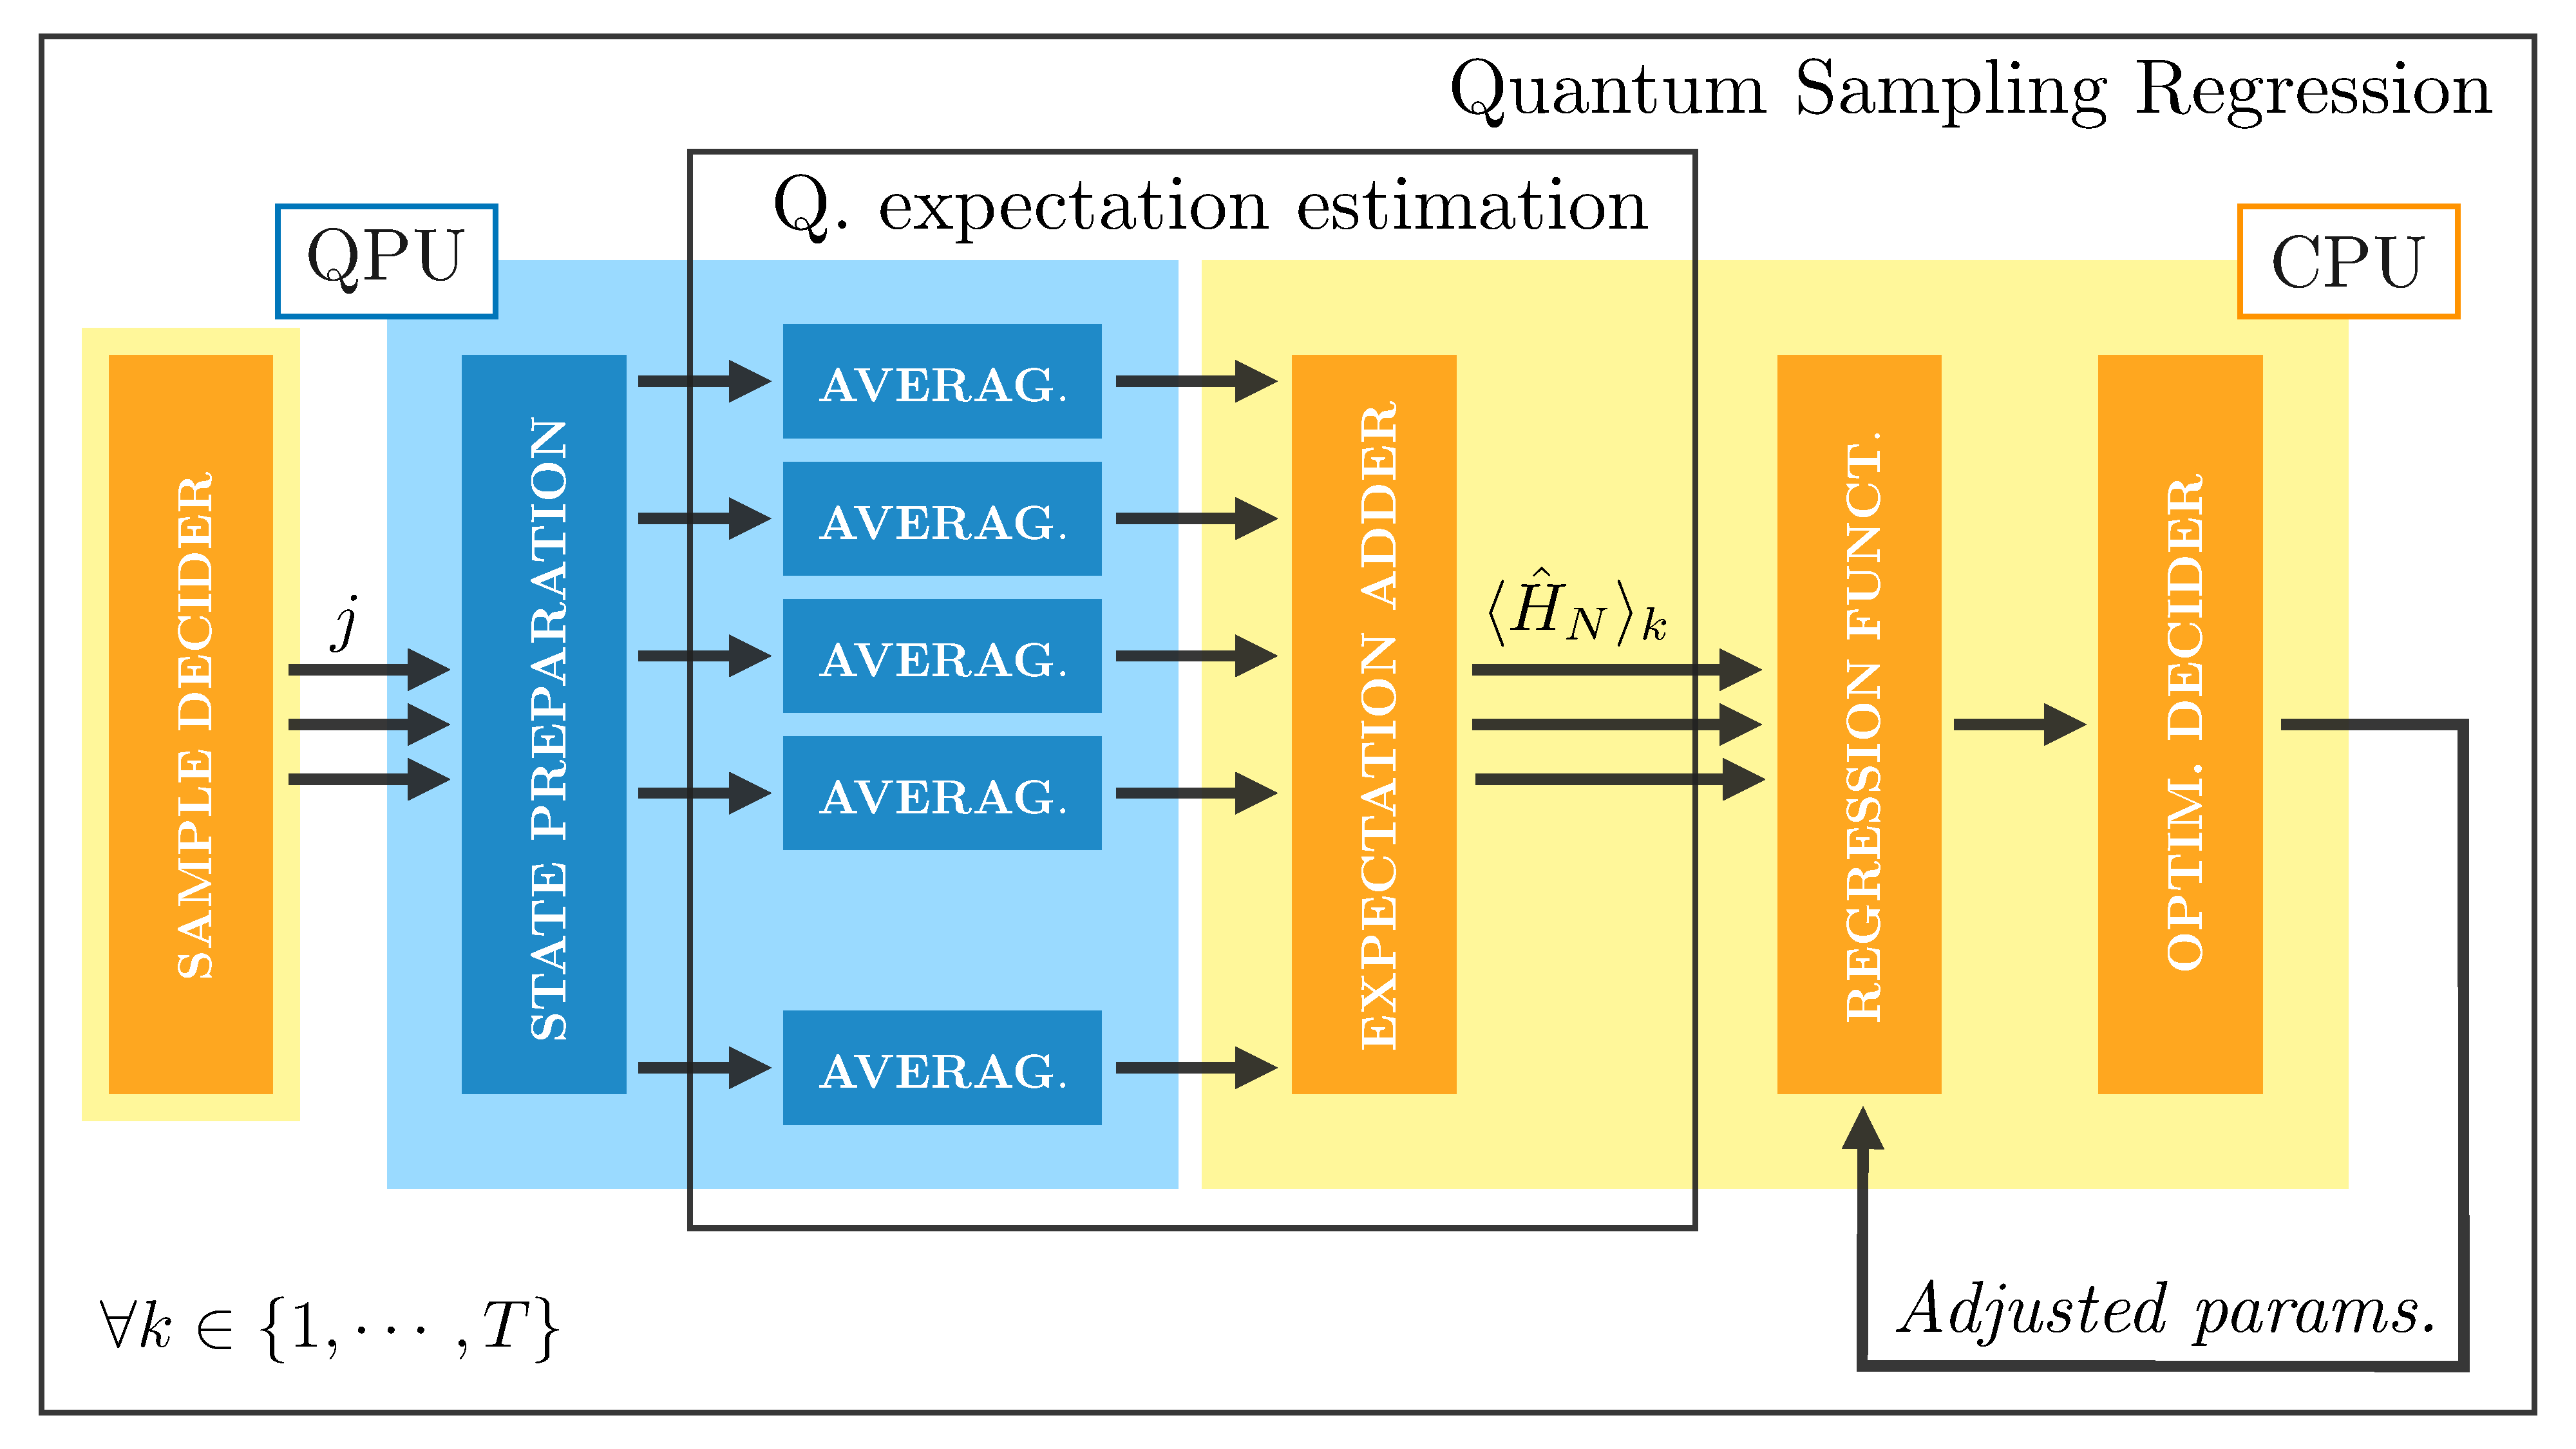
\includegraphics[width=1.0\linewidth]{Figures/QSR.pdf}
  \caption{Diagrammatic representation of the Quantum Sam-
  pling Regression algorithm (QSR).}
\end{figure}

\begin{block}{Introduction}

  \textbf{Variational quantum eigensolver} (VQE):
  \begin{enumerate}
    \item Prepare a quantum state in the quantum processor according to some parameters.
    \item Evaluate the expectation value of the computable addends in the target operator.
    \item Combine the previous expectation values by adding them up classically according to their respective weights.
    \item Use a classical optimization decider to generate a new set of parameters.
    \item Return to step one or stop if convergence has been reached.
  \end{enumerate}

  \begin{gather*} \label{eq:vqe-operator-averaging}
    \hat{H}_{N} = \sum_{j=1}^{\order{N^q}} w_{j} \hat{H}_{N}^{j} \qRa
    \ev{\hat{H}_{N}} = \sum_{j=1}^{\order{N^q}} w_{j} \ev{\hat{H}_{N}^{j}}
  \end{gather*}

  \vspace{1em}
  \begin{figure}
    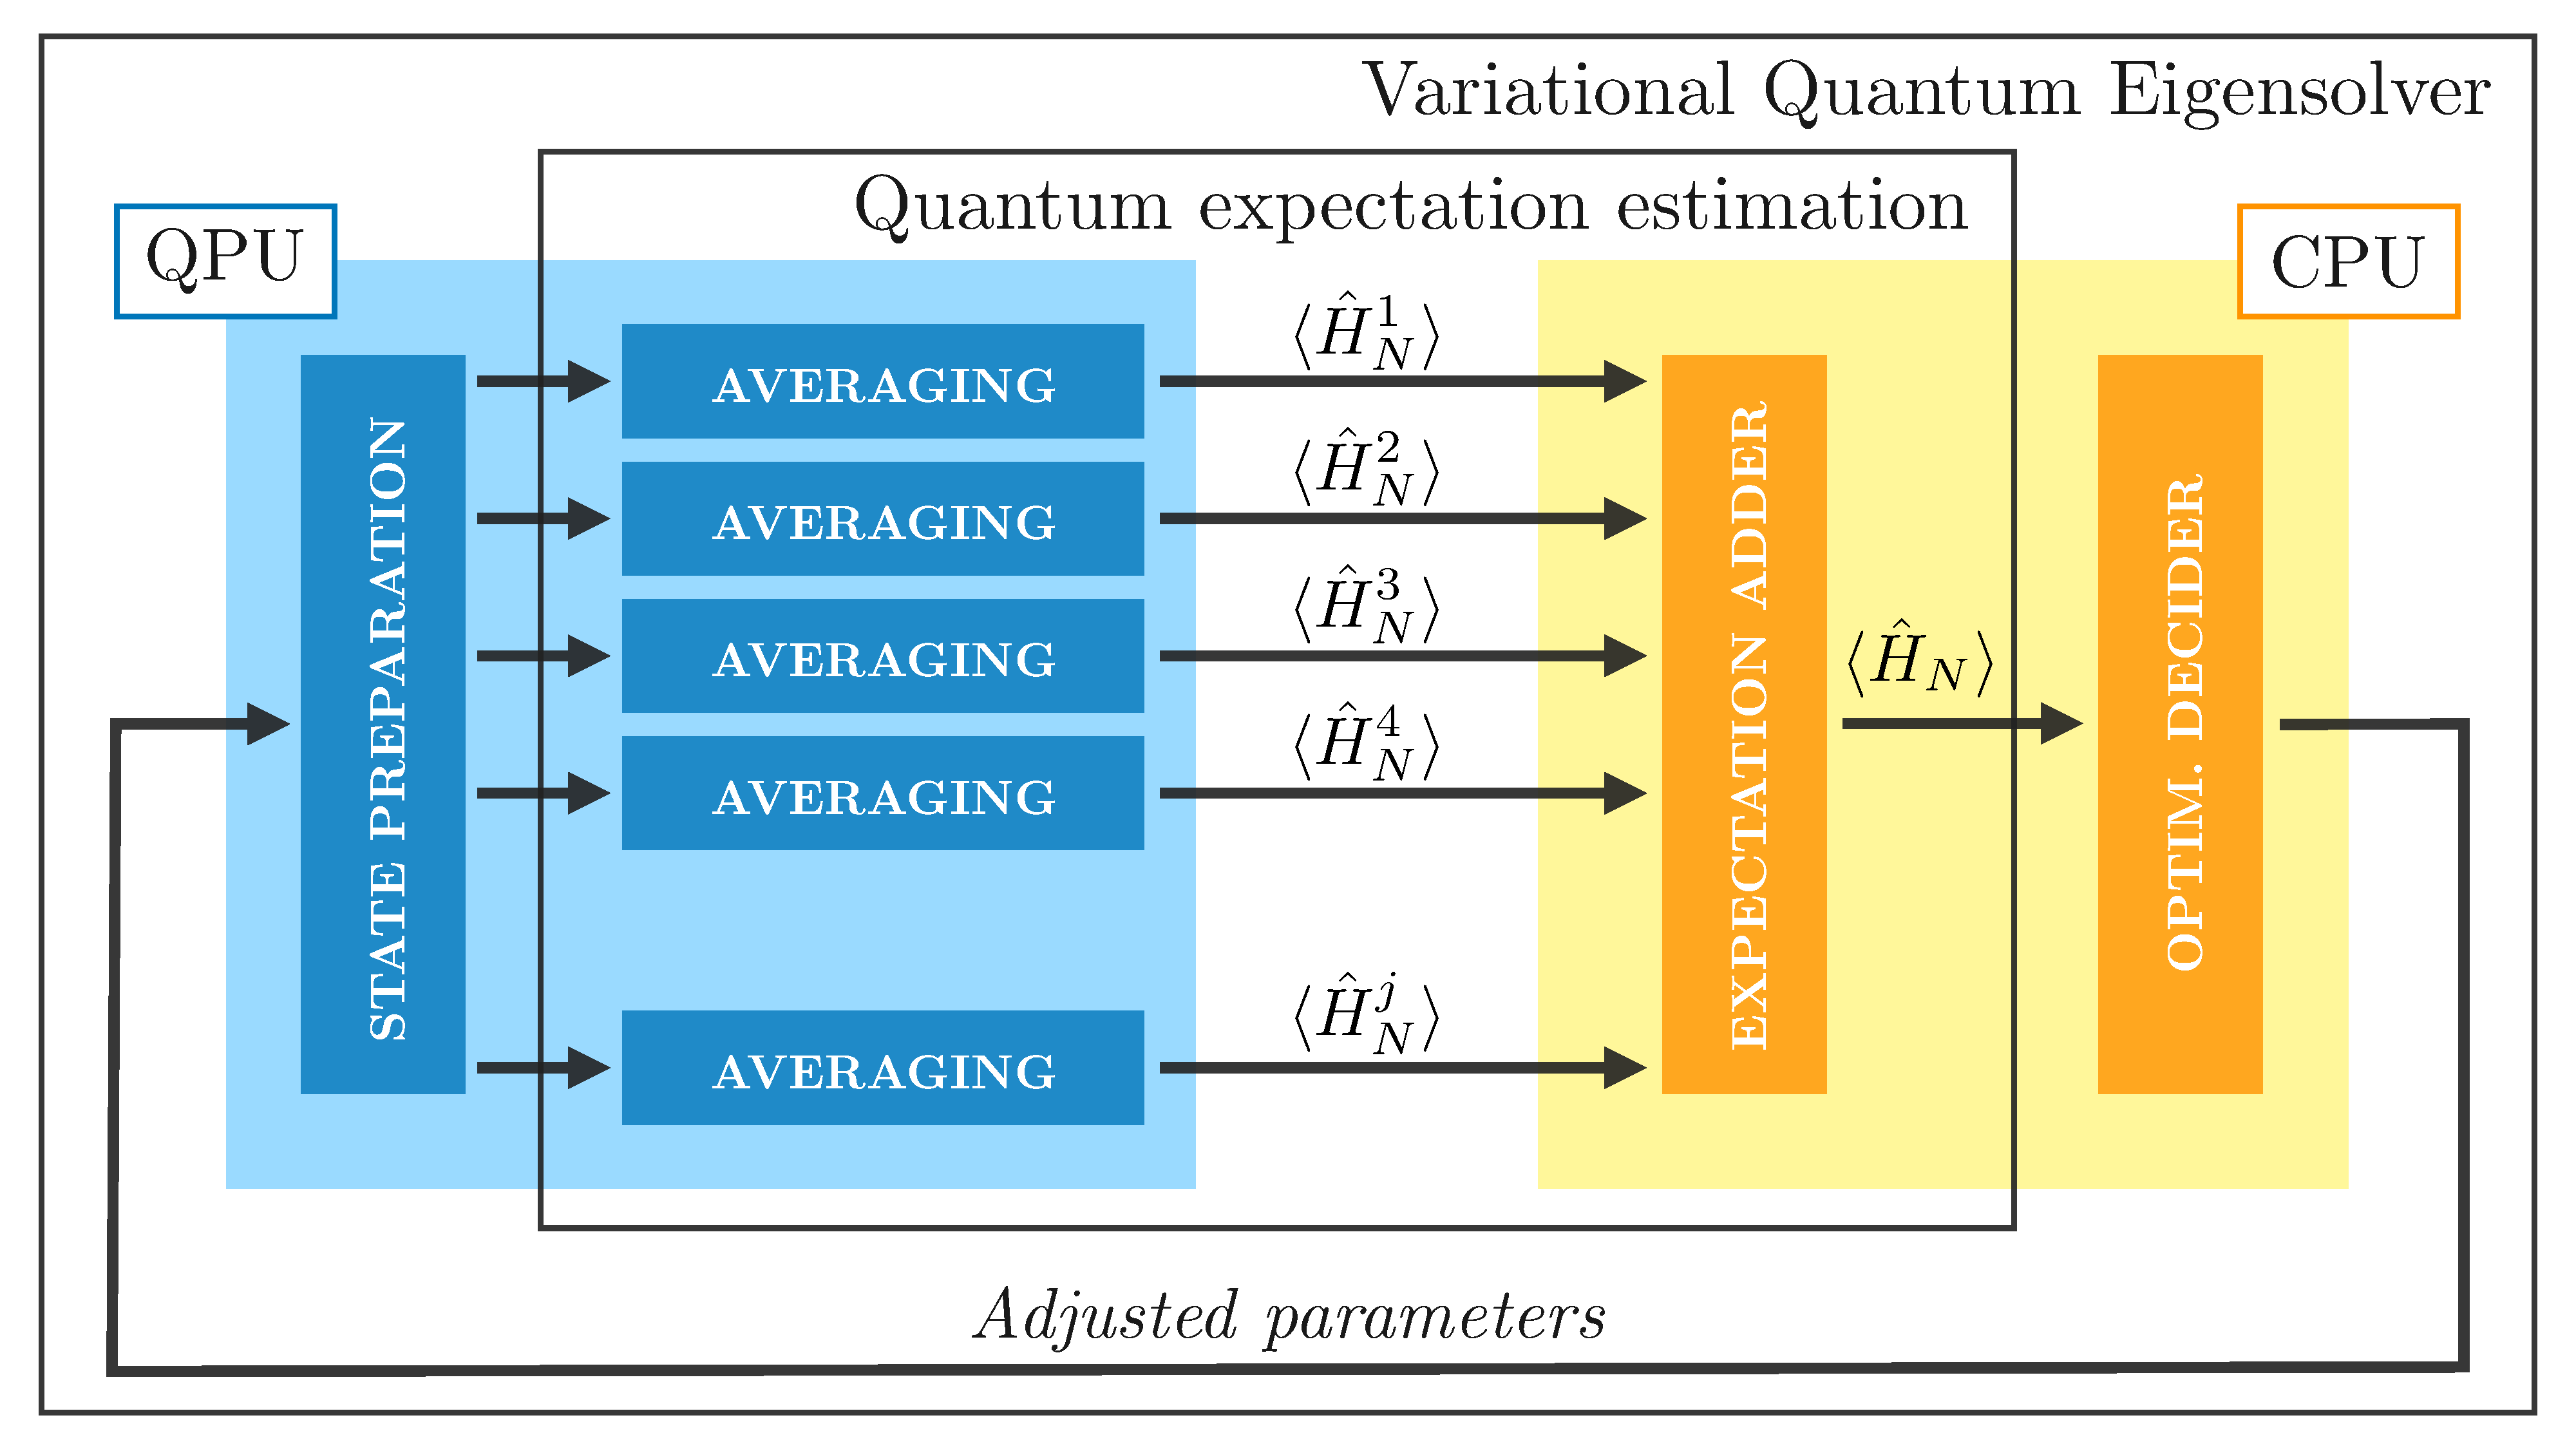
\includegraphics[width=1.0\linewidth]{Figures/VQE.pdf}
    \caption{Diagrammatic representation of the Variational Quantum Eigensolver algorithm (VQE).}
  \end{figure}

\end{block}

%% ----------------------------------------------------------------------------

\end{column} % End of the first column
\begin{column}{\sepwid}\end{column} % Empty spacer column
\begin{column}{\twocolwid} % Begin a column which is two columns wide (column 2)
\begin{columns}[t,totalwidth=\twocolwid] % Split up the two columns wide column
\begin{column}{\onecolwid}\vspace{-.6in} % First column within column 2 (2.1)

%% ----------------------------------------------------------------------------
%% ALGORTIHM OUTLINE
%% ----------------------------------------------------------------------------

\begin{block}{Algorithm outline}

  \textbf{Quantum sampling regression} (QSR):

  \begin{enumerate}
    \item Determine the bandwidth associated to each parameter in the parametrization ansatz.
    \item Sample the objective function using a quantum processor in the same way as for VQE.
    \item Compute the Fourier coefficients from the measured samples.
    \item In a classical machine, solve for the global minimum of the resulting regression function.
  \end{enumerate}

\end{block}

%% ----------------------------------------------------------------------------

\end{column} % End of column 2.1
\begin{column}{\onecolwid}\vspace{-.6in} % Second column within column 2 (2.2)

%% ----------------------------------------------------------------------------

\vspace{-1em}
\begin{gather*}
  h(\theta) \defeq \ev{\hat{H}_{N}}\qty(\theta) \equiv a_0 + \sum_{k=1}^S \qty[a_k\cos(k\theta) + b_k\sin(k\theta)]
\end{gather*}

\begin{gather*} \label{eq:QSR-algorithm-samples}
  T = \prod_{j=1}^{n} \qty(2 S_{j} + 1) \leq
    \qty(2 S_\text{max} + 1)^{n} \equiv 2^{sn}
\end{gather*}

\begin{alertblock}{Theoretical bedrock}
  \begin{itemize}
    \item \textbf{Quantum circuit topology} implies a frequency-bounded periodic domain.
    \item Fourier analysis: \textbf{Nyquist-Shannon sampling theorem} as proof of optimality.
  \end{itemize}
\end{alertblock}

%% ----------------------------------------------------------------------------

\end{column} % End of column 2.2
\end{columns} % End of the split of column 2 - any content after this will now take up 2 columns width

%% ----------------------------------------------------------------------------
%% PERFORMANCE COMPARISON
%% ----------------------------------------------------------------------------

\begin{alertblock}{Performance comparison}

  \begin{figure}
    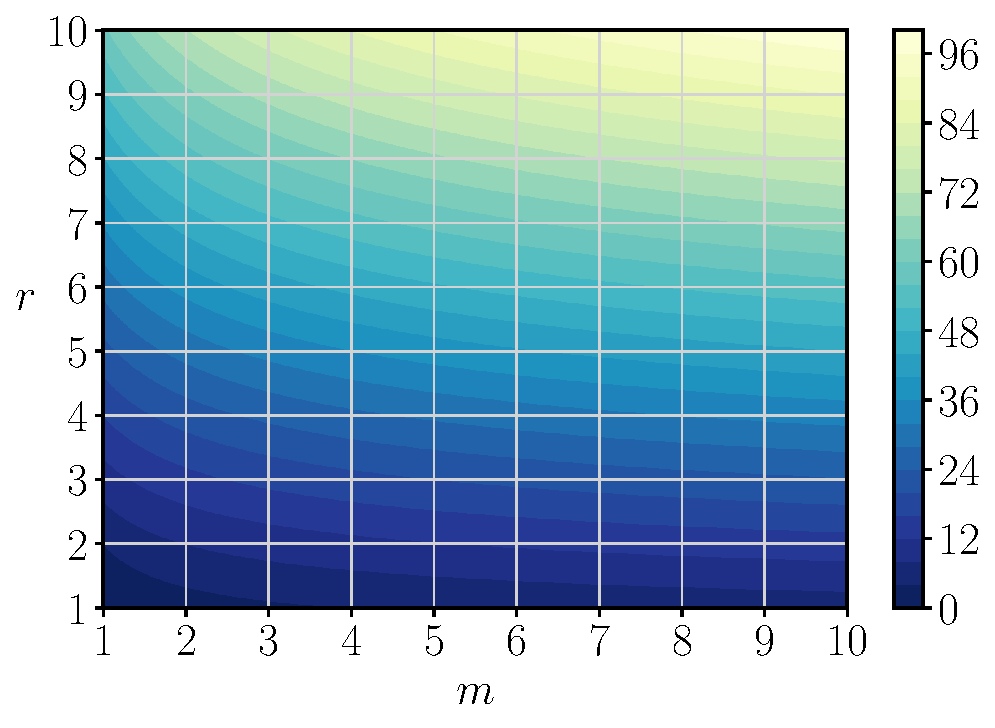
\includegraphics[width=0.4\linewidth]{Figures/threshold.pdf}
    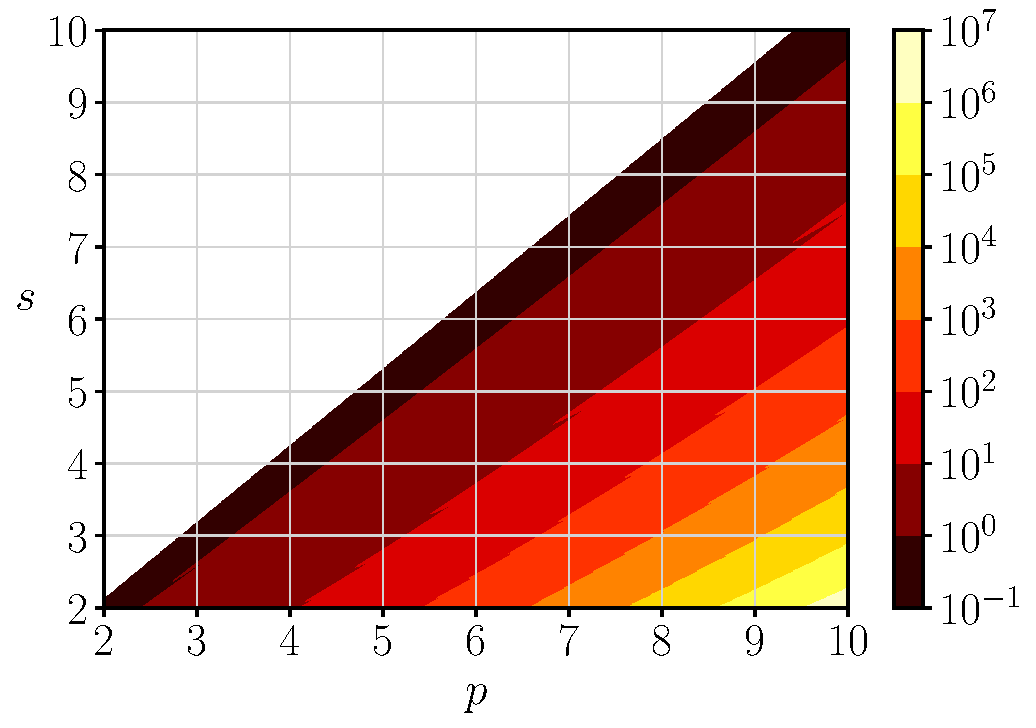
\includegraphics[width=0.4\linewidth]{Figures/efficiency.pdf}
    \caption{(Left) VQE threshold $a$. (Right) QSR average efficieny gains $E$ in the low qubit number regime.}
  \end{figure}

\end{alertblock}

%% ----------------------------------------------------------------------------

\begin{columns}[t,totalwidth=\twocolwid] % Split up into two columns again
\begin{column}{\onecolwid} % First column within column 2 (2.1)

%% ----------------------------------------------------------------------------
%% LOW QUBIT NUMBER REGIME
%% ----------------------------------------------------------------------------

\begin{block}{Low qubit number regime}

  Algorithmic complexity model:
  \begin{gather*}
    \frac{\textnormal{VQE}}{\textnormal{QSR}} = \qty(m n 2^{-n/r})^{p}
  \end{gather*}

  \vspace{1em}

  Threshold and average efficiency gains:
  \begin{gather*}
    a \defeq \ceil*{- \frac{r}{\ln{2}} W_{-1}\qty(-\frac{\ln{2}}{mr})} \\
    E \approx
      \frac{1}{as\ln{2}} \qty(\frac{m}{s\ln{2}})^p
      \Gamma \qty(p+1, s\ln{2}, as\ln{2}) \label{eq:QSR-efficiency}
  \end{gather*}

\end{block}

%% ----------------------------------------------------------------------------

\end{column} % End of column 2.1
\begin{column}{\onecolwid} % Second column within column 2 (column 2.2)

%% ----------------------------------------------------------------------------

\begin{figure}
  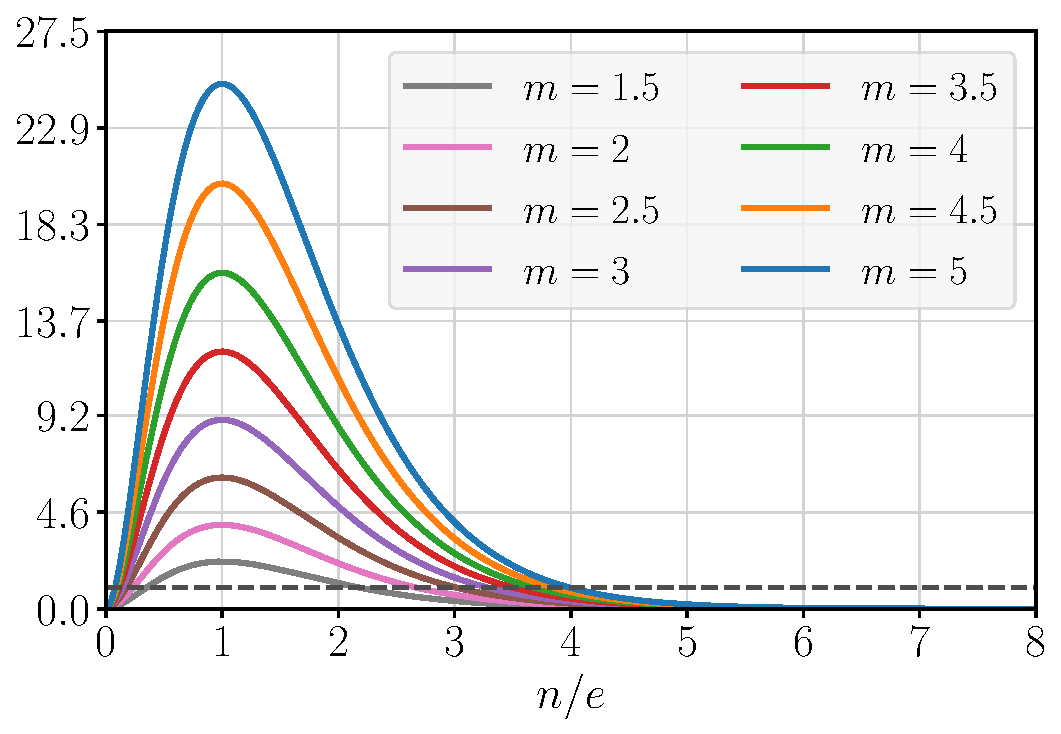
\includegraphics[width=0.9\linewidth]{Figures/VQE-vs-QSR_m.pdf}
  \caption{Comparison between the amount of quantum resources required by VQE and QSR with respect to the number of parameters in the ansatz.}
\end{figure}

%% ----------------------------------------------------------------------------

\end{column} % End of column 2.2
\end{columns} % End of the split of column 2
\end{column} % End of the second column
\begin{column}{\sepwid}\end{column} % Empty spacer column
\begin{column}{\onecolwid} % The third column

%% ----------------------------------------------------------------------------
%% APPLICATIONS
%% ----------------------------------------------------------------------------

\vspace{-2em}
\begin{figure}
  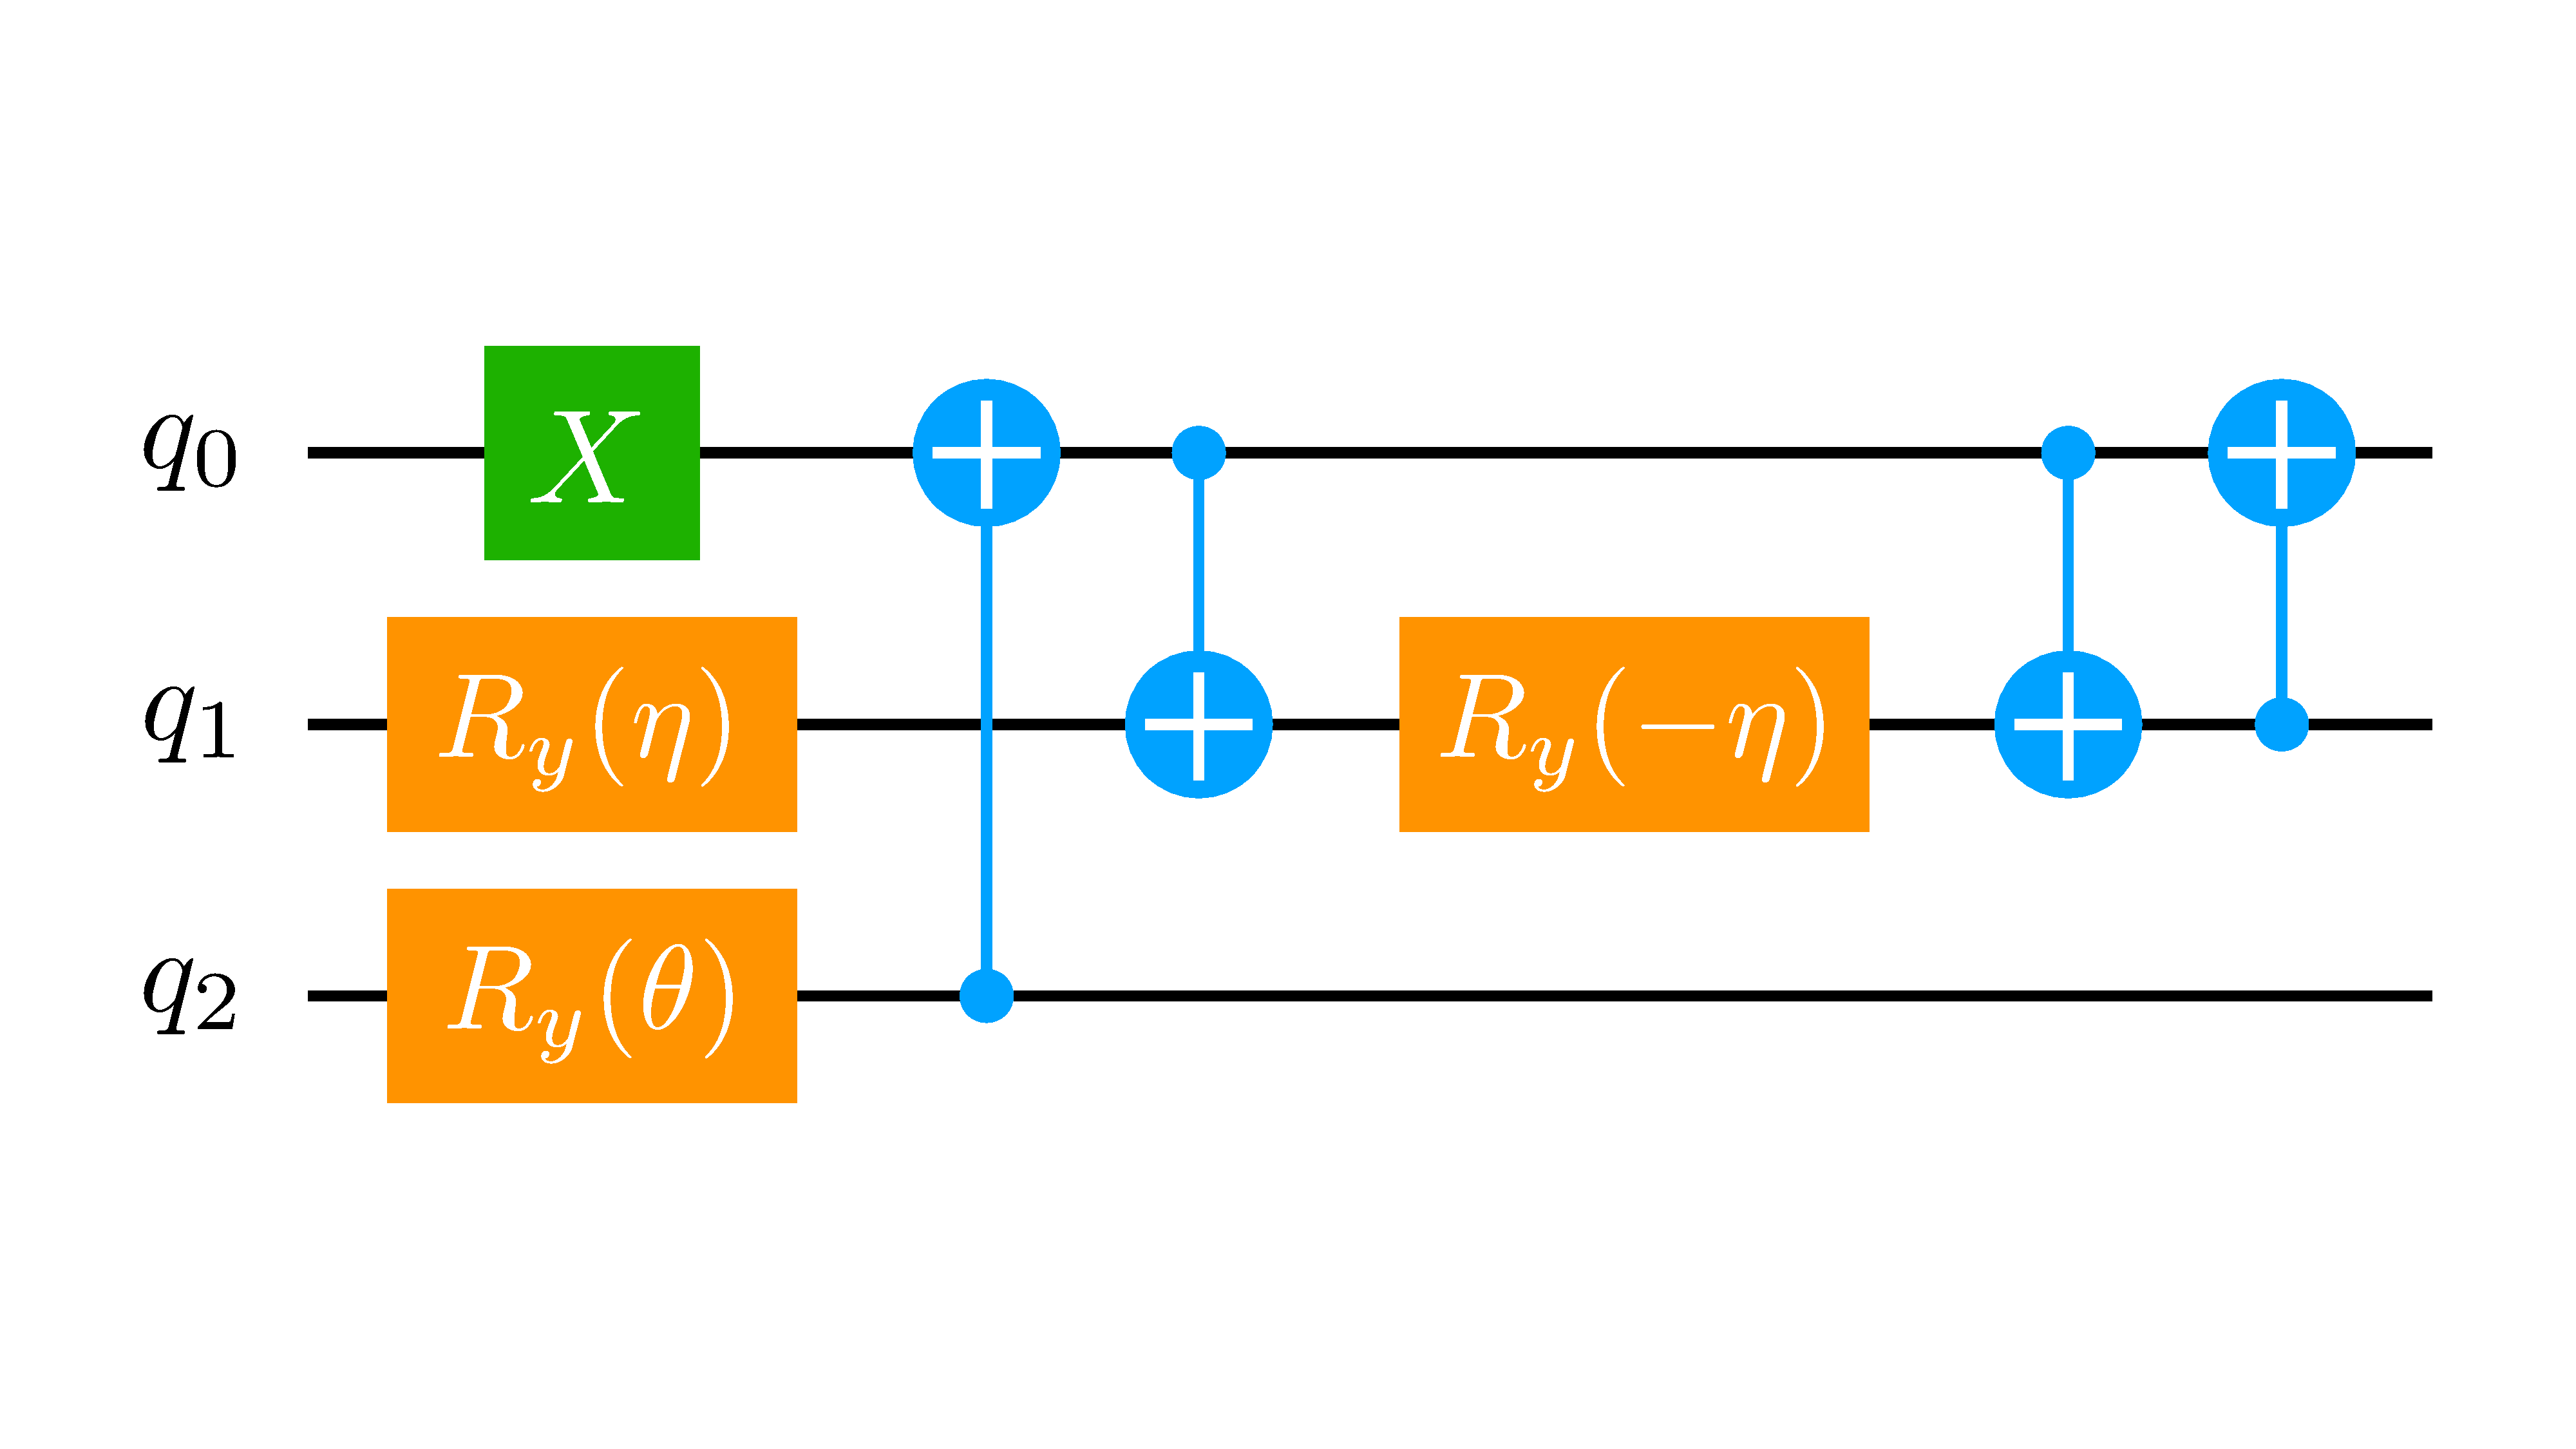
\includegraphics[width=0.8\linewidth]{Figures/quantum-circuit.pdf}
\end{figure}
\vspace{-2em}

\begin{block}{Applications}

  \begin{itemize}
    \item \textbf{Oversampling} to attain higher precision.
    \item \textbf{Undersampling} to boost performance and get rid of small-wavelength oscillations leading to burdensome local minima.
    \item VQE low-resolution start-up \textbf{supplement}.
    \item \textbf{Proxy} between simulators and real devices.
    \item Improve convergence by removing stochastic behavior, while retaining important features.
    \item Avoid the exponential matrix formulation in classical computation.
  \end{itemize}

\end{block}

%% ----------------------------------------------------------------------------
%% BENCHMARKING
%% ----------------------------------------------------------------------------

\begin{block}{Benchmarking}

  \vspace{-1em}
  \begin{table}[!bp]
  \caption{Comparison between results for the deuteron binding energy as reproduced using the VQE and QSR algorithms.\label{tab:vqe-qsr-comparison}}
    \bgroup
    \def\arraystretch{1.1}
    \setlength\tabcolsep{0.8em}
    \begin{tabular}{l l l l l}
    \toprule
    \toprule
    $n$ & Algorithm & Samples & Queries & Error \\
    \midrule
    $1$ & VQE & $24$ & $24$ & $3.5\%$ \\
    $1$ & QSR & $3$ & $1$ & $1.0\%$
  	\vspace{0.4em} \\
    $2$ & VQE & $183$ & $183$ & $0.3\%$ \\
    $2$ & QSR & $25$ & $1$ & $0.2\%$ \\
    \bottomrule
    \bottomrule
    \end{tabular}
    \egroup
  \end{table}

\end{block}

%% ----------------------------------------------------------------------------
%% REFERENCES
%% ----------------------------------------------------------------------------

% \begin{block}{References}
%
% \nocite{*} % Insert publications even if they are not cited in the poster
% \small{\bibliographystyle{unsrt}
% \bibliography{sample}\vspace{0.75in}}
% \vspace{-0.5in}
%
% \end{block}

%% ----------------------------------------------------------------------------
%% ACKNOWLEDGEMENTS
%% ----------------------------------------------------------------------------

\setbeamercolor{block title}{fg=RedOrange,bg=white} % Change block title color

\begin{block}{Acknowledgements}

  \begin{small}
  \begin{itemize}
    \item Chicago Quantum Exchange: Quantum Information Science and Engineering Network (\href{https://qisenet.uchicago.edu/overview/}{QISE- NET})
    \item U.S. Department of Energy, Office of Science, Office of Nuclear Physics, contract no. DE-AC02-06CH11357
  \end{itemize}
  \end{small}

\end{block}

%% ----------------------------------------------------------------------------
%% GENERAL INFORMATION
%% ----------------------------------------------------------------------------

% Change the alert block title colors
\setbeamercolor{block alerted title}{fg=black,bg=SpringGreen}
% Change the alert block body colors
\setbeamercolor{block alerted body}{fg=black,bg=white}

\begin{alertblock}{General Information}

  \begin{itemize}
    \item \textbf{Contact}: \href{mailto:priveroramirez@anl.gov}{priveroramirez@anl.gov}
    \item \textbf{ePrint}: \href{https://arxiv.org/abs/2012.02338}{arXiv:2012.02338}
  \end{itemize}

\end{alertblock}

%% ----------------------------------------------------------------------------

\end{column} % End of the third column
\end{columns} % End of all the columns in the poster
\end{frame} % End of the enclosing frame

%% ----------------------------------------------------------------------------

\end{document}
